\documentclass[a4paper,11pt]{article}

\usepackage[utf8]{inputenc}

\usepackage{graphicx}
\usepackage{caption}
\usepackage{subcaption}

\usepackage{pgfplots}
\pgfplotsset{compat=1.18} 

\usepackage{minted}
\usepackage{siunitx}

\begin{document}

\title{
    \textbf{Trees in C}
}
\author{Mo Wang}
\date{Spring 2026}

\maketitle

\section*{Introduction}

This report examines the performance and behavior of binary trees in C. A binary tree is a linked data structure that begins from the root node and stores two pointers to two other nodes, each of which in turn branches into two additional nodes. Ultimately nodes that do not divide to additional node branches are called leaf nodes. Conceptually, the tree is drawn from the root node on top, whereas it branches downward towards the leaf nodes. Each node branches into a left and a right node.

\section*{Binary tree}

\subsection*{Data structures}
A binary tree can be constructed using two structural components: a \emph{node block}, which stores an integer value together with pointers to its left and right child nodes, and a \emph{tree control block}, which stores a pointer to the root node. A leaf node is represented by a node block whose left and right child pointers are both \texttt{NULL}.

\begin{minted}{c}
typedef struct node {
    int value;
    struct node *right;
    struct node *left;
} node;

typedef struct tree {
    node *root;
} tree;
\end{minted}

\subsection*{Construct Node}
A node can be constructed by allocating it inside a tree, which can be done by dynamically allocating memory for the node and initializing its value.

\begin{minted}{c}
node *construct_node(int val) {
    node *nd = (node*) malloc(sizeof(node));
    
    if (!nd) {
        // Allocation failed; propagate NULL to the caller.
        // Caller should check for NULL and handle the error
        // (e.g., abort build, free partial tree).
        return NULL;
    }

    // Initialize fields
    nd->value = val;
    nd->left = NULL;
    nd->right = NULL;
    return nd;
}
\end{minted}

\subsection*{Free Node}
Freeing a node is not as straightforward as creating one, because it contains pointer addresses to other nodes, which would be lost in memory leakage if the node is simply removed. To address this, when a node is freed, the operation ensures that all nodes it points to are also freed. The \texttt{free\_node} function recursively frees the nodes, starting from a given node to prevent memory leaks.

\begin{minted}{c}
void free_node(node *nd) {
    // Freeing the nodes could be done recursively.
    if (nd != NULL) {
        free_node(nd->left);
        free_node(nd->right);
        free(nd);
    }
}
\end{minted}

\subsection*{Construct Tree}

The function \texttt{construct\_tree} allocates and initializes a new binary tree control block. The tree object contains a pointer to its root node, which is initially set to \texttt{NULL} to represent an empty tree. 
This function returns an empty heap-allocated \texttt{tree} control block that can subsequently be filled using insertion routines.

\begin{minted}{c}
tree *construct_tree() {
    tree *tr = (tree*) malloc(sizeof(tree));
    if (!tr) return NULL;  // Memory allocation failed.
    tr->root = NULL;
    return tr;
}
\end{minted}

\subsection*{Free Tree}
The function \texttt{free\_tree} releases all memory associated with a binary tree. It first invokes \texttt{free\_node} on the tree's root pointer, which recursively frees every node in the structure, and then deallocates the tree control block itself. After this call, the tree is fully destroyed and no allocated memory remains.

\begin{minted}{c}
void free_tree(tree *tr) {
    if (tr != NULL){
        free_node(tr->root);
        free(tr);
    }
}
\end{minted}

\section*{Sorted binary tree}

A sorted binary tree is a special case of a binary tree in which the nodes are organized according to a strict ordering rule. In this structure, each node stores an integer value, which enables direct comparison using the standard less-than and greater-than operators. For any given node, all values in its left subtree are strictly smaller than the value stored in the node, while all values in its right subtree are strictly larger. As a consequence, an in-order traversal of the tree yields the stored integers in sorted order, ranging from the leftmost node to the rightmost.

The two fundamental operations on a sorted binary tree are the insertion of a new integer value and the lookup of an existing one. Both operations must preserve the invariant that the left subtree contains smaller values and the right subtree contains larger values. Maintaining this ordering property is what allows the structure to support efficient searching while implicitly representing a sorted sequence.

\subsection*{Add operation}
Inserting new values into a binary search tree can be carried out using either a recursive strategy or an explicit iterative traversal, both of which must preserve the tree's ordering invariant.

\subsubsection*{Add operation with recursion}
An insertion operation can be implemented recursively by beginning from the root node and comparing the insertion value to its current node value. If the insertion value is equal to the node value, no insertion operation is performed, as duplicated values are not allowed. However, if the inserted value is less than the node value, the left node will be proceeded, otherwise, the right node will be traversed, where the process starts over. As the leaf node is reached, the value is attached to the suitable branch, either left or right depending on the leaf node value.

\begin{minted}{c}
node* add_node(node *nd, int value){
    // if node is not constructed.
    if (nd == NULL){
        return construct_node(value); // returns NULL on allocation failure
    }

    // Recurse into the appropriate branch to maintain BST ordering.
    if (value < nd->value) {
        nd->left = add_node(nd->left, value);
    } else if (value > nd->value) {
        nd->right = add_node(nd->right, value);
    } else {
        // value == nd->value — duplicate value; by convention to do nothing.
    }
    return nd;
}

void recursive_add(tree *tr, int value){
    // If tree is NULL, there is nowhere to insert.
    if (tr == NULL) {
        return;
    }
    // Insert and reassign in case the root becomes newly created.
    tr->root = add_node(tr->root, value);
    // If add_node operation fails, root node pointer address remains NULL,
    // which should be checked after calling recursive_add function
}
\end{minted}

\subsubsection*{Add operation without recursion}

The insert operation can also be implemented without recursion. In this case, traversal down each depth level can be maintained by current node variable \texttt{nd} and parent node variable \texttt{parent}. The algorithm starts from the root node and traverses the tree by comparing the insertion value with the current node value. Depending on the value being smaller or larger than the insertion value, the algorithm moves to left or right child, updating both \texttt{parent} and \texttt{nd} variables, until an appropriate leaf node is reached. At that point, the new node is attached as a left or right child, depending on the value of the parent node.

Since the non-recursive implementation omits function call and additional stack frame push on each depth traversal, the performance, both time and space, is generally better than recursive implementation, given the same binary tree.

\begin{minted}{c}
void add(tree *tr, int value) {
    if (tr == NULL) {
        return; // No tree to insert into (defensive check).
    }

    node *parent = NULL;      // Tracks the parent of the position.
    node *nd     = tr->root;  // Current node while descending the tree.

    // Descend until we find a NULL position where the new node should go.
    while (nd != NULL) {
        parent = nd;
        if (value < nd->value) {
            nd = nd->left;      // go left
        } else if (value > nd->value) {
            nd = nd->right;     // go right
        } else {
            // value == nd->value  -> duplicate; by convention, do nothing.
            return;
        }
    }

    // Create the new leaf node once the insertion point is found.
    node *new_node = construct_node(value);
    if (new_node == NULL) {
        // Allocation failed; the tree remains unchanged.
        return;
    }

    // If the tree was empty, the new node becomes the root.
    if (parent == NULL) {
        tr->root = new_node;
        return;
    }

    // Attach the new node as the appropriate child of 'parent'.
    if (value < parent->value) {
        parent->left = new_node;
    } else {
        parent->right = new_node;
    }
}
\end{minted}

\subsubsection*{Theoretical time complexity}
The time complexity is proportional to the depth of the tree, since the algorithm has to traverse down to the leaf node before a value can be attached. The depth can vary in different cases. The best case is a well-balanced tree with $n$ nodes, resulting into $\log_2(n)$ depth and logarithmic time complexity $O(\log n)$. However, in the worst case, the tree can degenerate into a linked list with $n$ depth, resulting in linear time complexity $O(n)$.

\subsection*{Lookup procedure}
The lookup procedure determines whether a given value exists in the binary search tree by traversing the structure according to the BST ordering rules.

\subsubsection*{Implementation}
The lookup procedure can, in the simplest form, be implemented with recursion. In each tree depth traversal, the search value is compared with the node value. If the value is the same as the node value, the value is already found. Otherwise, depending on whether the search value is smaller or greater than the node’s value, the procedure is recursively repeated in the left or right sub-tree, respectively, until the leaf node is reached to decide whether the value exists in the tree.

\begin{minted}{c}
bool lookup_node(node *nd, int value){
    // If empty subtree, value not present.
    if (nd == NULL) return false;
    
    if (value < nd->value) {
        // If value is smaller: search left subtree.
        return lookup_node(nd->left, value);
    } else if (value > nd->value) {
        // If value is larger: search right subtree.
        return lookup_node(nd->right, value);
    } else {
        // value == nd->value → found it.
        return true;
    }
}

bool recursive_lookup(tree *tr, int value){
    // If the tree pointer is NULL, the value cannot be found.
    if (tr == NULL) return false;

    return lookup_node(tr->root, value);
}
\end{minted}

\subsubsection*{Theoretical time complexity}

The running time of a lookup operation in a binary search tree is directly proportional to the depth of the path taken from the root to the target node. Because the depth of a binary tree depends on how well its values are structured, lookup performance can vary significantly between different insertion patterns. In the best case, when the tree is relatively balanced, the height grows proportionally to $\log_2(n)$ for $n$ nodes, yielding an efficient lookup complexity of $O(\log n)$. In the worst case, inserting values in sorted order causes the tree to degenerate into a linear chain of nodes, which has height $n$ and therefore results in a linear-time lookup complexity of $O(n)$. These two contrasting shapes are illustrated in Figure~\ref{fig:balanced-vs-unbalanced}: a balanced tree achieves shallow height, whereas an unbalanced one with all right children mirrors the behavior of a linked list.

\begin{figure}[h]
  \centering

  \begin{subfigure}[t]{0.48\textwidth}
    \centering
    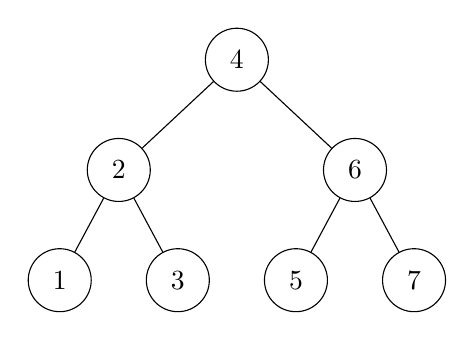
\begin{tikzpicture}[
        level distance=1.4cm,
        every node/.style={circle,draw,minimum size=8mm},
        level 1/.style={sibling distance=30mm},
        level 2/.style={sibling distance=15mm}
    ]
    \node {4}
        child { node {2}
            child { node {1} }
            child { node {3} }
        }
        child { node {6}
            child { node {5} }
            child { node {7} }
        };
    \end{tikzpicture}
    \subcaption{Balanced binary tree}
    \label{fig:balanced}
  \end{subfigure}
  \hfill
  \begin{subfigure}[t]{0.48\textwidth}
    \centering
    \begin{tikzpicture}[
        level distance=1cm,
        every node/.style={circle,draw,minimum size=8mm},
        level 1/.style={sibling distance=25mm},
        level 2/.style={sibling distance=25mm},
        level 3/.style={sibling distance=25mm},
    ]
    \node {1}
      child [missing]
      child { node {2}
        child [missing]
        child { node {...}
          child [missing]
          child { node {7} }
        }
      };
    \end{tikzpicture}
    \subcaption{Fully unbalanced (all right children)}
    \label{fig:unbalanced}
  \end{subfigure}

  \caption{Balanced vs.\ unbalanced binary trees placed side by side.}
  \label{fig:balanced-vs-unbalanced}
\end{figure}

\subsubsection*{Benchmark}
To validate these theoretical bounds, a lookup benchmark was conducted across three different insertion patterns: inserting values to intentionally build a well-balanced tree, inserting values in sorted order to construct an unbalanced tree, and inserting a shuffled sequence of integers to approximate a typical average-case behavior. The lookup measurements are shown in Table~\ref{tab:bst-lookup-complexity}, and their growth trends are plotted in Figure~\ref{fig:bst-lookup-complexity}. The results clearly show that the balanced tree provides the lower performance bound, following an $O(\log n)$ trend, while the unbalanced tree exhibits linear growth consistent with $O(n)$. The shuffled-input tree lies between these two extremes. Although it occasionally behaves closer to the balanced case, deviations from perfect balance can cause temporary increases in depth and corresponding performance overheads.

\begin{table}[h]
  \centering
  \begin{tabular}{r|r|r|r}
    \textbf{N} & \textbf{BST\_balanced}
               & \textbf{BST\_shuffled}
               & \textbf{BST\_unbalanced} \\ \hline
     1024   & 9   & 19   & 1\,070   \\
     2048   & 12  & 19   & 2\,102   \\
     4096   & 13  & 32   & 4\,068   \\
     8192   & 17  & 42   & 8\,331   \\
    16384   & 28  & 62   & 15\,484  \\
    32768   & 27  & 55   & 33\,935  \\
    65535   & 33  & 71   & 66\,598  \\
   131072   & 38  & 84   & 182\,722 \\
  \end{tabular}
  \caption{Balanced vs.\ shuffled vs.\ unbalanced BST lookup times (ns).}
  \label{tab:bst-lookup-complexity}
\end{table}

% Preamble:
% \usepackage{pgfplots}
% \pgfplotsset{compat=1.18}

\begin{figure}[h]
  \centering
  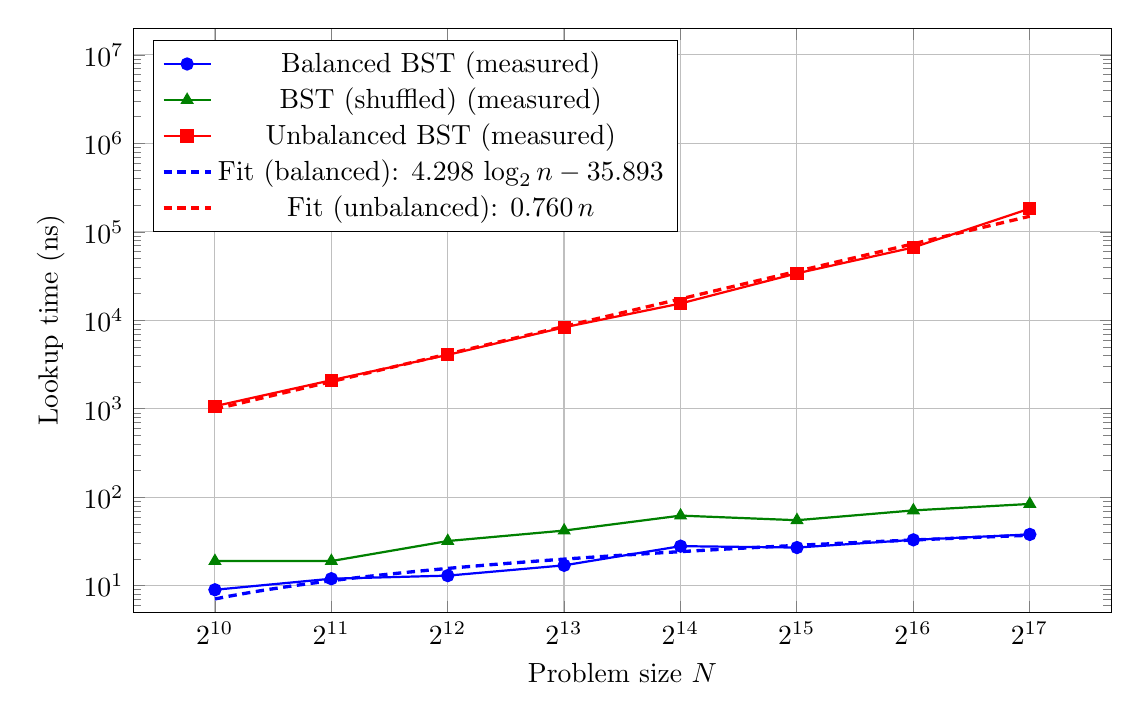
\begin{tikzpicture}
    \begin{axis}[
      xmode=log,
      ymode=log,
      log basis x=2,                 % base-2 for the N axis (optional but nice)
      xlabel={Problem size $N$},
      ylabel={Lookup time (ns)},
      width=14cm, height=9cm,
      grid=major,
      legend style={at={(0.02,0.98)}, anchor=north west, draw=black, fill=white},
      xmajorgrids=true, ymajorgrids=true,
      ymin=5, ymax=2e7               % > 0 for log-scale; headroom for the top point
    ]

      % -------------------------------
      % Balanced BST (measured)
      % -------------------------------
      \addplot[color=blue, mark=*, thick] coordinates {
        (1024,9)
        (2048,12)
        (4096,13)
        (8192,17)
        (16384,28)
        (32768,27)
        (65535,33)
        (131072,38)
      };
      \addlegendentry{Balanced BST (measured)}

      % -------------------------------
      % Shuffled BST (measured)
      % -------------------------------
      \addplot[color=green!50!black, mark=triangle*, thick] coordinates {
        (1024,19)
        (2048,19)
        (4096,32)
        (8192,42)
        (16384,62)
        (32768,55)
        (65535,71)
        (131072,84)
      };
      \addlegendentry{BST (shuffled) (measured)}

      % -------------------------------
      % Unbalanced BST (measured)
      % -------------------------------
      \addplot[color=red, mark=square*, thick] coordinates {
        (1024,1070)
        (2048,2102)
        (4096,4068)
        (8192,8331)
        (16384,15484)
        (32768,33935)
        (65535,66598)
        (131072,182722)
      };
      \addlegendentry{Unbalanced BST (measured)}

      % -----------------------------------------
      % Fitted line for Balanced BST (logarithmic model):
      %   t(n) ≈ 4.2976 * log2(n) - 35.8929   [R^2 ≈ 0.954]
      % Note: On a log–log axis this is slightly curved (expected).
      % -----------------------------------------
      \addplot[
        blue,
        densely dashed,
        very thick,
        domain=1024:131072,
        samples=60
      ] {4.2976246104 * (ln(x)/ln(2)) - 35.8929204138};
      \addlegendentry{Fit (balanced): $4.298\,\log_{2}n - 35.893$}

      % -----------------------------------------
      % Fitted line for Unbalanced BST (power law on log–log axes):
      %   t(n) ≈ 0.7604 * n^{1.0347}          [R^2 ≈ 0.997]
      % -----------------------------------------
      \addplot[
        red,
        densely dashed,
        very thick,
        domain=1024:131072,
        samples=60
      ] {0.7604219238 * (x^1.0347020881)};
      \addlegendentry{Fit (unbalanced): $0.760\,n$}

    \end{axis}
  \end{tikzpicture}

  \caption{Balanced, shuffled, and unbalanced BST lookup times (ns) on log--log axes with fitted lines (logarithmic model for balanced; power-law model for unbalanced).}
  \label{fig:bst-lookup-complexity}
\end{figure}

In summary, the lookup operation in a binary search tree exhibits a wide range of possible running times depending on the shape of the tree. A well-balanced tree achieves the optimal logarithmic behavior, while a pathologically constructed tree grows linearly. Empirical measurements confirm that real-world performance falls between these extremes, with shuffled inputs typically producing moderately balanced trees whose lookup times approximate $O(\log n)$ but occasionally deviate when temporary imbalances occur.

\subsubsection*{Comparison with binary search algorithm}

In a balanced BST (best case), the lookup operation has a time complexity of $O(\log n)$. This corresponds to a tree height of $\log_2(n)$ and closely resembles the behavior of binary search in an array, where each comparison determines which half of the array to inspect next. However, binary search poses a larger arithmetic overhead, especially calculating the middle value with clock cycle consuming division, and is therefore slower compared to BST lookup that relies on direct pointer adress accessing in memory.

Table~\ref{tab:bst-binary-search-complexity} and
Figure~\ref{fig:bst-binary-search-complexity} show that BST lookup consistently achieves better performance. Although both algorithms relies on pointer chasing, BST lookup in a well-balanced tree significantly outperforms binary search without the excessive index calculation overhead.

\begin{table}[h]
  \centering
  \begin{tabular}{r|r|r}
    \textbf{N} & \textbf{lookup\_ns(BST)} & \textbf{lookup\_ns(binsearch)} \\ \hline
     1024   &  9  & 33 \\
     2048   & 12  & 40 \\
     4096   & 13  & 46 \\
     8192   & 17  & 52 \\
    16384   & 28  & 57 \\
    32768   & 27  & 66 \\
    65535   & 33  & 75 \\
   131072   & 38  & 86 \\
  \end{tabular}
  \caption{Lookup times (ns) for a well-balanced BST and array binary search.}
  \label{tab:bst-binary-search-complexity}
\end{table}

% Preamble:
% \usepackage{pgfplots}
% \pgfplotsset{compat=1.18}

\begin{figure}[h]
  \centering
  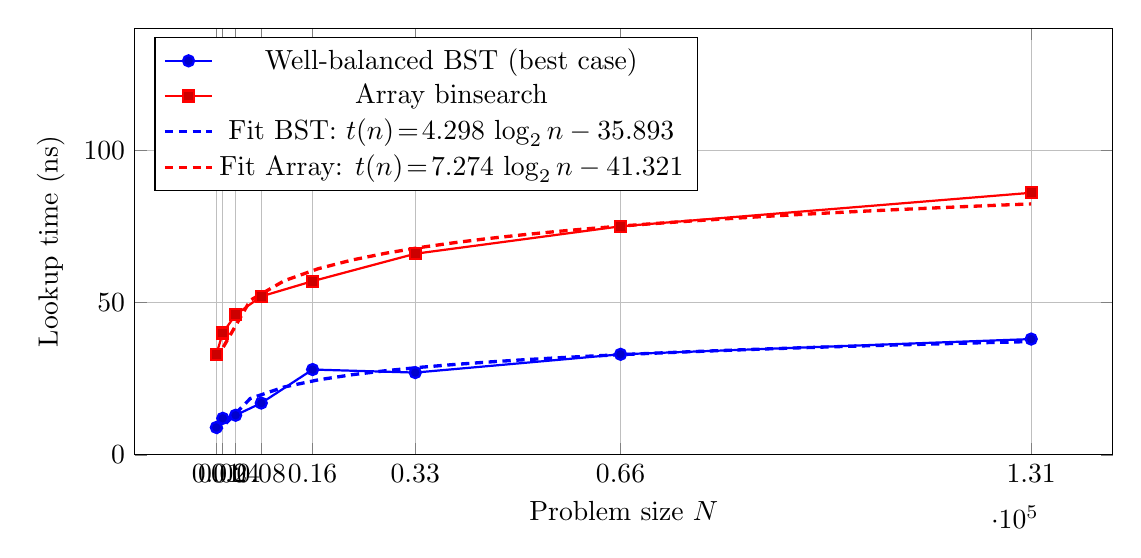
\begin{tikzpicture}
    \begin{axis}[
      xlabel={Problem size $N$},
      ylabel={Lookup time (ns)},
      width=14cm, height=7cm,
      grid=major,
      ymajorgrids=true,
      xmajorgrids=true,
      clip=true,
      ymin=0, ymax=140,                 % tight range to show small ns values clearly
      xtick={1024,2048,4096,8192,16384,32768,65536,131072},
      xticklabel style={/pgf/number format/fixed},
      legend style={at={(0.02,0.98)}, anchor=north west, draw=black, fill=white}
    ]

      % ----------------------------------------------------------------
      % Measured data: Balanced BST
      % ----------------------------------------------------------------
      \addplot+[
        mark=*,
        thick,
        color=blue
      ] coordinates {
        (1024,  9)
        (2048, 12)
        (4096, 13)
        (8192, 17)
        (16384,28)
        (32768,27)
        (65536,33)
        (131072,38)
      };
      \addlegendentry{Well-balanced BST (best case)}

      % ----------------------------------------------------------------
      % Measured data: Array binary search
      % ----------------------------------------------------------------
      \addplot+[
        mark=square*,
        thick,
        color=red
      ] coordinates {
        (1024,  33)
        (2048,  40)
        (4096,  46)
        (8192,  52)
        (16384, 57)
        (32768, 66)
        (65536, 75)
        (131072,86)
      };
      \addlegendentry{Array binsearch}

      % ----------------------------------------------------------------
      % Fitted O(log2 N) line for BST (least-squares on your data)
      %   t(n) ≈ 4.297619... * log2(n) - 35.892857...   (R^2 ≈ 0.954)
      % ----------------------------------------------------------------
      \addplot[
        blue,
        densely dashed,
        very thick,
        domain=1024:131072,
        samples=25
      ] {4.2976190476 * (ln(x)/ln(2)) - 35.8928571429};
      \addlegendentry{Fit BST: $t(n)\!=\!4.298\,\log_{2}n-35.893$}

      % ----------------------------------------------------------------
      % Fitted O(log2 N) line for Array (least-squares on your data)
      %   t(n) ≈ 7.273809... * log2(n) - 41.321428...   (R^2 ≈ 0.985)
      % ----------------------------------------------------------------
      \addplot[
        red,
        densely dashed,
        very thick,
        domain=1024:131072,
        samples=25
      ] {7.2738095238 * (ln(x)/ln(2)) - 41.3214285714};
      \addlegendentry{Fit Array: $t(n)\!=\!7.274\,\log_{2}n-41.321$}

    \end{axis}
  \end{tikzpicture}
  \caption{Lookup benchmark: well-balanced BST vs array binary search (ns) with $O(\log_{2}N)$ fits.}
  \label{fig:bst-binary-search-complexity}
\end{figure}

As the tree becomes unbalanced, the time complexity degrades towards $O(n)$, as the depth level approaches the number of elements in the array $n$. In contrast, the binary search on the sorted array remains unaffected by structural imbalance, consistently maintaining a time complexity of $O(\log(n))$. Thus, the binary search in an array generally outperforms the binary search algorithm in an unbalanced binary search tree.

\section*{Depth first traversal}

The depth first traversal is a collective of traversal algorithms that traverses down to one of the leaf nodes of the tree before backtracking and visiting other branches. These algorithms comprises \emph{in-order traversal}, as well as \emph{pre-order} and \emph{post-order traversal}.

\subsection*{In-order traversal}

An in-order depth first traversal starts with the root node and recursively traverses the left sub-tree, processes the current node, and then traverses the right sub-tree. It can easily be built using recursion by pushing the current depth onto the implicit stack during each recursive call, while popping it up when returning back to that depth. 

This in-order traversal algorithm is particular useful for printing the elements of the binary search tree in sorted sequence order, as the left-most node is visited and printed first, followed by the nodes in middle towards the right-most node. The sorted sequence is guaranteed since the left branch of each node contains smaller values while the right branch contains larger values. The \texttt{print\_tree} function starts with the tree root node, and recursively traverses it while printing out the elements of the tree using the helper function \texttt{print}.

\begin{minted}{c}
static void print(node *nd) {
    // Omit if node pointer address holds NULL
    if (nd != NULL) {
        print(nd->left); // Visit left branch first
        printf("%d ", nd->value); // Process node value
        print(nd->right); // Visit right branch
    }
}

void print_tree(tree *tr) {
    if (tr->root != NULL)
        // Visit root
        print(tr->root);
    printf("\n");
}
\end{minted}

\subsection*{Pre-order traversal}
Pre-order traversal starts with processing the root node, before traversing the left and right subbranches. The traversal algorithm is particularly useful when the node on higher depth has higher precedence than its children node.

Pre-order traversal is shown below using print function as an example.

\begin{minted}{c}
static void print(node *nd) {
    if (nd != NULL) {
        printf("%d ", nd->value); // Process node value
        print(nd->left); // Visit left branch first
        print(nd->right); // Visit right branch
    }
}
\end{minted}

\subsection*{Post-order traversal}
Post-order traversal is similar to pre-order traversal, but processes the left and right subtrees before processing the root node. This traversal is often used in scenarios where the children nodes must be processed before the parent node, for example, recursively removing a subbranch of a tree which is used previously in \texttt{free\_tree} operation for deallocating a tree.

Post-order traversal is shown below using print function as an example.

\begin{minted}{c}
static void print(node *nd) {
    if (nd != NULL) {
        print(nd->left); // Visit left branch first
        print(nd->right); // Visit right branch
        printf("%d ", nd->value); // Process node value
    }
}
\end{minted}

\section*{Traversal using explicit stack}
\subsection*{Stack}
The depth first traversal of a tree can also be implemented using an explicit stack instead of relying on the implicit programming stack during each recursive call. On each traversal, instead of recursive function call when stepping down a tree depth, the current stack depth is stored into an explicit stack by pushing a tree node pointer address.

\begin{minted}{c}
typedef struct stack {
    node **elements;
    size_t capacity;
    size_t top; /* index of next free slot */
} stack;
\end{minted}

The dynamic stack implemented in earlier assignments is used to store pointers to nodes encountered during tree traversal. It supports the fundamental operations required for an explicit-stack in-order traversal. The stack provides:

\begin{itemize}
    \item \texttt{static stack *stack\_create()}  
          -- Allocates and initializes an empty dynamic stack.

    \item \texttt{static void stack\_free(stack *stk)}  
          -- Deallocates all internal memory associated with the stack.

    \item \texttt{static void stack\_push(stack *stk, node *nd)}  
          -- Pushes a node pointer onto the top of the stack.

    \item \texttt{static bool stack\_empty(const stack *stk)}  
          -- Returns \texttt{true} if the stack contains no elements.

    \item \texttt{static node *stack\_pop(stack *stk)}  
          -- Removes and returns the node pointer from the top of the stack.
\end{itemize}

\subsection*{Explicit-stack in-order traversal}
In-order traversing using an explicit stack can be implemented by initially traversing down from the root to the left-most leaf node, while nodes pointers are pushed to the stack. In this case, as the left sub-tree of a node being popped from the stack has been processed, the node itself needs to be processed before the values of the right sub-tree needs to be processed. By processing the right sub-tree, the left-most node of the right subbranch is traversed before processing the rest elements. This process is repeated until the root node is reached and there are no more stack depths above, which can be detected by checking the stack being empty.

Using this approach, the binary search tree can be printed using in-order traversal, where the node value is printed when a node is processed.

\begin{minted}{c}
void tree_print_inorder_stack(const tree *tr) {
    stack *stk = stack_create();
    node *nd = tr->root;

    /* move to leftmost path initially */
    while (nd != NULL) {
        stack_push(stk, nd);
        nd = nd->left;
    }

    while (!stack_empty(stk)) {
        node *nd = stack_pop(stk);
        printf("%d ", nd->value);  /* left handled, now visit node */

        /* then handle right subtree: push its left path */
        node *r = nd->right;
        while (r != NULL) {
            stack_push(stk, r);
            r = r->left;
        }
    }
    stack_free(stk);
    printf("\n");
}
\end{minted}

\subsection*{Practical advantages of explicit-stack traversal}

Although the in-order traversal implemented with an explicit stack produces the same output as the recursive version, the explicit stack can offer functional advantages that the implicit programming stack cannot provide. In the recursive approach, the traversal state - that is, the sequence of pending nodes yet to be processed - is managed automatically and cannot be inspected, modified, or stored by the programmer. In contrast, when using an explicit stack, the traversal state is fully accessible and can therefore be preserved, resumed, or manipulated. This becomes useful in scenarios where we want to pause a traversal at a specific node and later continue from exactly that position, or when we need to describe or reuse the sequence of remaining elements after a certain point in the traversal. While this additional control adds no particular benefit for the simple print example, it provides valuable flexibility in more advanced applications such as lazy iteration, tree-based search algorithms, and custom traversal strategies.

\section*{Conclusion}

This report has examined the construction, operational, and performance characteristics of binary trees in C, with a focus on sorted binary search trees (BST) and their traversal mechanisms. By implementing both recursive and iterative variants of the tree operations - node construction, insertion, lookup, and deallocation - the report demonstrates how the shape and the structure of a tree directly affects its runtime behavior.

The benchmark experiments clearly show that the time efficiency of a BST tree depends heavily on its structural balance. A well‑balanced BST produces the desired logarithmic behavior, enabling fast lookup and insertion operations. However, when values are inserted in sorted order, the tree degenerates into a linked‑list‑like structure, resulting in linear‑time performance. Shuffled input however does not guarantee perfectly balanced tree, but the produced BST trees can still achieve near‑logarithmic performance on average.

Comparing BST lookup with array binary search further conforms how memory layout structure affects performance. Although the two implementations share similar complexity in the balanced case, the BST lookup in a well-balanced tree outperforms the binary search due to the absence of a calculation of the array indices, which is described in Figure~\ref{tab:time-complexity-comparaison}

\begin{table}[h]
  \centering
  \begin{tabular}{l|c|p{5.2cm}}
    \textbf{Operation}
      & \textbf{Time}
      & \textbf{Notes} \\ \hline

    \textbf{BST lookup (balanced)}
      & $O(\log n)$
      & Requires specified input or self‑balancing structure (e.g. AVL/Red‑Black). \\ \hline

    \textbf{BST lookup (unbalanced)}
      & $O(n)$
      & Tree shape depends on insertion order; may degrade into a list. \\ \hline

    \textbf{Binary search}
      & $O(\log n)$
      & Always balanced; uses contiguous memory. \\ \hline

  \end{tabular}
  \caption{Time complexity comparison of search operations.}
  \label{tab:time-complexity-comparaison}
\end{table}

Finally, the exploration of depth‑first traversal using both recursion and an explicit stack shows how traversal strategies influence flexibility. Although the recursive version is more compact and less verbose in code, the explicit‑stack approach exposes intermediate traversal state and enables advanced use cases that recursion cannot support.

Overall, the study illustrates not only how binary trees can be implemented effectively in C, but also why their performance must be understood in the context of tree shape, data patterns, and memory organization.

\end{document}